% Drawing 148/01-13 -- folder 148, batch 01, archive page 17 (PDF page 18).
% Transcription: plus bas, un grand tétraèdre aux quatre sommets tronqués (de petites ellipses brunes), arêtes vertes et brunes, l'arête cachée en tirets bruns ; à l'intérieur, en vert, deux graphes en forme de H joignant les quatre trous, l'un en trait plein épais, l'autre en pointillé.
% Kind: truncated tetrahedron with two H-shaped graphs (pants decompositions). Method 2 (schematic redraw from the facsimile). Status: ok.
% Notes: Colour scan. The four vertices are cut off by small brown ellipses (holes), each with three heavy points where the edges arrive; beyond each hole the pencil tip of the uncut tetrahedron (three faint strokes from the tip to the three points). Edges between the holes: top-left, top to bottom right and right to bottom right in brown; top-right and left to bottom right in green, heavy; the hidden edge left-right in brown dashes. Inside, in heavy green: a broken line from the left face (on the top-left edge) across to the right edge, joined by a vertical stroke to the top hole and by a short stroke down to the bottom-right hole (an H: the holes top and bottom right on one side). In dotted green: from the left end of the broken line and from the left hole two rows of dots meeting at a junction, a row from there to the right edge, and a row from the right hole down to it (the second H, holes left and right). Not named in the notes of the transcription, whose « grand tétraèdre tronqué » mixes this figure with the one above (01-12). Redrawn 2026-11-12 (issue 128). 2026-11-13, Claude Opus 5.5, issue 147, overlay check: not compiled (no TeX in the session); the TikZ was rasterised by a local interpreter and laid over the 236 ppi scan rendered at 400 dpi. Redrawn on the ink: holes fitted as ellipses on their ink, points on the centres of their blots, edges and green strokes fitted by least squares; every stroke lies on its ink to within about one unit. Changed: holes and edges moved onto the ink (they were up to three units off); each edge now ends on the points of its holes; the pencil tips beyond the holes are drawn; the dotted green strokes are drawn as rows of round dots spaced as on the page, along their own routes (the junction of the two rows from the left, then on to the right edge). Only the number and phase of the green dots are TikZ's, not the page's.
% Coordinates: 1 unit = 1 mm = 1/100 of the crop width, y downwards as on the crop (bbox in page fractions: [0.08, 0.515, 0.66, 0.775]).
% Redrawn by Claude (claude-fable-5-2), issue #128, 2026-11-12; not checked by a human; not compiled (no TeX in the session); overlay-checked on the scan by Claude Opus 5.5, issue #147, 2026-11-13, not compiled (no TeX in the session).
% Rights: reproduces part of the work -- behind RENDER_TRANSCRIPTS, never published by itself.
\documentclass[tikz,border=3pt]{standalone}
\usepackage{amsmath,amssymb}
\usetikzlibrary{patterns,arrows.meta}
\tikzset{pencil/.style={black!45}, struck/.style={black!35}, mpt/.style={circle,draw,inner sep=1.3pt}, pt/.style={circle,fill,inner sep=0.9pt}, opt/.style={circle,draw,fill=white,inner sep=1.1pt}, Rd/.style={red!75!black}, Gn/.style={green!45!black}, Br/.style={brown!70!black}}
\begin{document}
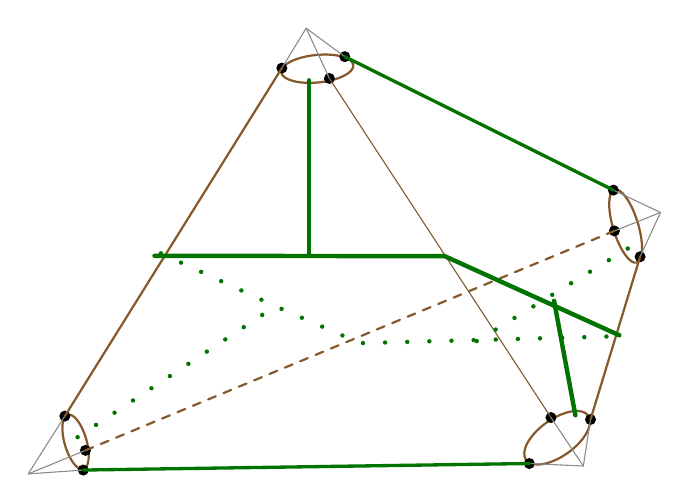
\begin{tikzpicture}[x=1mm,y=-1mm,line cap=round,line join=round,font=\small]
% the four holes (small brown ellipses cutting off the vertices), each with three points where the edges arrive
\draw[Br,thick,rotate around={5.6:(52.31,6.44)}] (52.31,6.44) ellipse [x radius=4.6, y radius=1.75];
\draw[Br,thick,rotate around={-73:(91.47,26.43)}] (91.47,26.43) ellipse [x radius=4.85, y radius=1.6];
\draw[Br,thick,rotate around={-73.9:(21.61,53.84)}] (21.61,53.84) ellipse [x radius=3.6, y radius=1.4];
\draw[Br,thick,rotate around={35.5:(82.77,53.31)}] (82.77,53.31) ellipse [x radius=4.85, y radius=2.35];
\foreach \p in {(47.81,6.36),(55.8,4.91),(53.85,7.68),(89.91,21.86),(90.04,27.04),(93.31,30.32),(20.25,50.56),(22.87,54.91),(22.59,57.41),(79.24,56.58),(81.99,50.74),(87.01,50.99)} {\fill \p circle [radius=0.7];}
% the pencil tips of the uncut tetrahedron beyond the holes
\draw[pencil] (20.25,50.56) -- (15.6,57.9) -- (22.59,57.41);
\draw[pencil] (15.6,57.9) -- (22.87,54.91);
\draw[pencil] (89.91,21.86) -- (95.9,24.7) -- (93.31,30.32);
\draw[pencil] (95.9,24.7) -- (90.04,27.04);
\draw[pencil] (47.81,6.36) -- (50.9,1.3) -- (55.8,4.91);
\draw[pencil] (50.9,1.3) -- (53.85,7.68);
\draw[pencil] (81.99,50.74) -- (86.1,56.9) -- (79.24,56.58);
\draw[pencil] (86.1,56.9) -- (87.01,50.99);
% edges between the holes: brown (top-left, top-bottom right, right-bottom right), green (top-right, left-bottom right), the hidden one in brown dashes
\draw[Br,thick] (47.81,6.36) -- (20.25,50.56);
\draw[Br] (53.85,7.68) -- (81.99,50.74);
\draw[Br,thick] (93.31,30.32) -- (87.01,50.99);
\draw[Gn,very thick] (55.8,4.91) -- (89.91,21.86);
\draw[Gn,very thick] (22.59,57.41) -- (79.24,56.58);
\draw[Br,thick,dashed] (22.87,54.91) -- (90.04,27.04);
% the solid green H: a broken line from the left face to the right edge, a stroke up to the top hole and one down to the bottom right hole
\draw[Gn,line width=1.6pt] (31.64,30.2) -- (68.5,30.25) -- (90.68,40.3);
\draw[Gn,line width=1.6pt] (51.24,7.92) -- (51.24,30.2);
\draw[Gn,line width=1.6pt] (82.38,35.92) -- (85.09,50.46);
% the dotted green H: from the left end of the broken line and from the left hole to a junction, on to the right edge, and from the right hole down to it
\draw[Gn,line width=1.6pt,dash pattern=on 0pt off 8pt] (32.45,29.89) -- (47,36.6) -- (57.75,41.3) -- (90.8,40.41);
\draw[Gn,line width=1.6pt,dash pattern=on 0pt off 8pt] (21.87,53.23) -- (47,36.6);
\draw[Gn,line width=1.6pt,dash pattern=on 0pt off 8pt] (91.74,29.28) -- (72.45,41.1);
\end{tikzpicture}
\end{document}
